\section{Probability}

\mode<presentation>{
%---------------------------------------------------------------------slide----
\begin{frame}
\frametitle{Probability}
\tableofcontents[sectionstyle=show/hide,hideothersubsections]
\end{frame}
}


%---------------------------------------------------------------------slide----
\begin{frame}
\frametitle{Introduction}
Descriptive Statistics provide methods to describe de variables measured in the sample and their relations, but it
doesn't allow to draw any conclusion about the population.

Now it's time to make the leap from the sample to the population and the bridge for that is the
\highlight{probability theory}.

Remember that the sample has a limited information about the population, and in order to draw valid conclusions for the
population the sample must be representative of it.
For that reason, to guarantee the representativeness of the sample, this must be drawn randomly. 
This means that the choice of individuals in the sample is by chance. 

The probability theory will give us the tools to control the random in the sampling and to determine the level of
reliability of the conclusions drawn from the sample. 
\end{frame}


\subsection{Random experiments and events}

%---------------------------------------------------------------------slide----
\begin{frame}
\frametitle{Random experiments}
The study of a characteristic of the population is conducted through random experiments. 

\begin{definition}[Random experiment] A \emph{random experiment} is an experiment that meets two conditions:
\begin{enumerate}
\item It is known the set of possible outcomes. 
\item It is impossible to predict the outcome with absolute certainty.
\end{enumerate} 
\end{definition}

\textbf{Example}. Gambling are typical examples of random experiments. 
The roll of a dice, for example, is a random experiment cause
\begin{itemize}
\item It is known the the set of possible outcomes: $\{1,2,3,4,5,6\}$.
\item Before rolling the dice, it's impossible to predict with absolute certainty the face of the dice that will occur. 
\end{itemize}

Another non-gambling example is the random choice of an individual of a human population and the determination of its
blood type. 
Generally, the draw of a sample by a random method  is an random experiment.
\end{frame}


%---------------------------------------------------------------------slide----
\begin{frame}
\frametitle{Sample space}
\begin{definition}[Sample space]
The set $\Omega$ of the possible outcomes of a random experiment is known as \emph{sample space}.
\end{definition}

\textbf{Example} Some examples of sample spaces are:
\begin{itemize}
\item For the toss of a coin $\Omega=\{heads,tails\}$.
\item For the roll of a dice $\Omega=\{1,2,3,4,5,6\}$.
\item For the blood type of an individual drawn by chance $\Omega=\{\mbox{A},\mbox{B},\mbox{AB},\mbox{0}\}$.
\item For the height of an individual drawn by chance $\Omega=\mathbb{R}^+$.
\end{itemize}
\end{frame}


%---------------------------------------------------------------------slide----
\begin{frame}
\frametitle{Sample space construction}
In experiments where more than one variable is measured, the determination of the sample space can be difficult. 
In such a cases, it is advisable to use a \highlight{tree diagram} to construct the sample space. 

In a tree diagram every variable is represented in a level of the tree and every possible outcome of the variable as a
branch.
\end{frame}


%---------------------------------------------------------------------slide----
\begin{frame}
\frametitle{Sample space construction}
\framesubtitle{Example of gender and blood type}
% The tree below represents the sample space of a random experiment where we measure the gender and the blood type of a
% person.

\begin{center}
\tikzsetnextfilename{probability/sample_space}
\resizebox{0.8\textwidth}{!}{% Author: Alfredo Sánchez Alberca (asalber@ceu.es)

\begin{tikzpicture}[
grow'=right,
% sloped,
level 1/.style ={level distance=2cm, sibling distance=3.2cm, parent anchor=east, child anchor=west},
level 2/.style ={level distance=4cm, sibling distance=0.8cm},
level 3/.style ={level distance=2cm, sibling distance=0.8cm, dashed}
]

\node (root) {}
	child {
		node {Female}
    	child {node {0}
				child {node{(Female,0)}}
			}
 			child {node {A}
				child {node{(Female,A)}}
			}
			child {node {B}
				child {node{(Female,B)}}
			}
			child {node {AB}
				child {node{(Female,AB)}}
			}
    }
	child {
		node {Male}
    	child {node {0}
				child {node{(Male,0)}}
			}
 			child {node {A}
				child {node{(Male,A)}}
			}
			child {node {B}
				child {node{(Male,B)}}
			}
			child {node {AB}
				child {node{(Male,AB)}}
			}
    };

\begin{scope}[every node/.style={text width=2cm, align=center, anchor=center, font=\bfseries,}]
\node[above= 0.5cm of root-1-1-1] (labels-level) {$\Omega$};
\node[at =(labels-level-|root-1-1)] {Blood type};
\node[at =(labels-level-|root-1)] {Gender};
\end{scope}
\end{tikzpicture}

}
\end{center}
\end{frame}


%---------------------------------------------------------------------slide----
\begin{frame}
\frametitle{Random events}
\begin{definition}[Random event]
A \emph{random event} is any subset of the sample space $\Omega$ of a random experiment.
\end{definition}

There are different types of events:
\begin{itemize}
\item \textbf{Impossible event:} Is the event with no elements $\emptyset$. It has no chance of occurring.
\item \textbf{Elemental events:} Are events with only one element, that is, a singleton.
\item \textbf{Composed events:} Are events with two or more elements.
\item \textbf{Sure event:} Is the event that contains the whole sample space. It always happens.
\end{itemize}
\end{frame}


\subsection{Set theory}

%---------------------------------------------------------------------slide----
\begin{frame}
\frametitle{Event space}
\begin{definition}[Event space] Given a sample space $\Omega$ of a random experiment, the \emph{event space} of
$\Omega$ is the set of all possible events of $\Omega$, and is noted $\mathcal{P}(\Omega)$.
\end{definition}

\textbf{Example}. Given the sample space $\Omega=\{a,b,c\}$, its even space is 
\[
\mathcal{P}(\Omega)=\left\{\emptyset, \{a\},\{b\},\{c\},\{a,b\},\{a,c\},\{b,c\},\{a,b,c\}\right\}
\]
\end{frame}


%---------------------------------------------------------------------slide----
\begin{frame}
\frametitle{Event operations}
As events are subsets of the sample space, using the set theory we have the following operations on events:
\begin{itemize}
\item Union
\item Intersection
\item Complement
\item Difference
\end{itemize}
\end{frame}


% ---------------------------------------------------------------------slide----
\begin{frame}
\frametitle{Union of events}
\begin{definition}[Union event]
Given two events $A,B\in \mathcal{P}(\Omega)$, the \emph{union} of $A$ and $B$, denoted by $A\cup B$, is the event of
all elements that are members of $A$ or $B$ or both.
\[
A\cup B = \{x\,|\, x\in A\textrm{ or }x\in B\}.
\]
\end{definition}

\begin{center}
\tikzsetnextfilename{probability/union}
% Author: Alfredo Sánchez Alberca (asalber@ceu.es)

\begin{tikzpicture}
\def\firstcircle{(1.5,1.5) circle (1cm)}
\def\secondcircle{(2.5,1.5) circle (1cm)}

\fill[color1!30] \firstcircle;
\fill[color1!30] \secondcircle;
\draw (0,3) node[anchor=north east] {$\Omega$} rectangle (4,0);
\draw \firstcircle node[xshift=-0.9cm, yshift=0.9cm] {$A$};
\draw \secondcircle node[xshift=0.9cm, yshift=0.9cm] {$B$};

\node at (2,0.3) {$A\cup B$};
\end{tikzpicture}
\end{center}
The union event $A\cup B$ happens when $A$ \alert{or} $B$ happen.
\end{frame}


%---------------------------------------------------------------------slide----
\begin{frame}
\frametitle{Intersection of events}
\begin{definition}[Intersection event]
Given two events $A,B\in \mathcal{P}(\Omega)$, the \emph{intersection} of $A$ and $B$, denoted by $A\cap B$, is the
event of all elements that are members of both $A$ and $B$.
\[
A\cap B = \{x\,|\, x\in A\textrm{ and }x\in B\}.
\]
\end{definition}

\begin{center}
\tikzsetnextfilename{probability/intersection}
% Author: Alfredo Sánchez Alberca (asalber@ceu.es)

\begin{tikzpicture}
\def\firstcircle{(1.5,1.5) circle (1cm)}
\def\secondcircle{(2.5,1.5) circle (1cm)}

\begin{scope}
\clip \firstcircle;
\fill[color1!30] \secondcircle;
\end{scope}

\draw (0,3) node[anchor=north east] {$\Omega$} rectangle (4,0);
\draw \firstcircle node[xshift=-0.9cm, yshift=0.9cm] {$A$};
\draw \secondcircle node[xshift=0.9cm, yshift=0.9cm] {$B$};

\node at (2,1.5) {$A\cap B$};
\end{tikzpicture}
\end{center}
The intersection event $A\cap B$ happens when $A$ \alert{and} $B$ happen.

% Observe that the intersection event is included in the union even $A\cap B \subseteq A\cup B$.

Two events are \highlight{incompatible} if their intersection is empty.
\end{frame}


%---------------------------------------------------------------------slide----
\begin{frame}
\frametitle{Complement of an event}
\begin{definition}[Complementary event]
Given an event $A\in \mathcal{P}(\Omega)$, the \emph{complementary or contrary event} of $A$, denoted by $\bar A$, is
the event of all elements of $\Omega$ except the elements that are members of $A$.
\[
\overline A = \{x\,|\, x\not\in A\}.
\]
\end{definition}

\begin{center}
\tikzsetnextfilename{probability/complement}
% Author: Alfredo Sánchez Alberca (asalber@ceu.es)

\begin{tikzpicture}
\def\circle{(1.5,1.5) circle (1cm)}
\def\rectangle{(4,0) rectangle (0,3)}

\begin{scope}[even odd rule]
\clip \circle (0,0) rectangle (4,3);
\fill[color1!30] \rectangle;
\end{scope}

\draw \rectangle node[anchor=north east] {$\Omega$};
\draw \circle node {$A$};
\node at (3,1.5) {$\overline A$};
\end{tikzpicture}
\end{center}

The complementary event $\bar A$ happens when $A$ does \alert{not} happen.
\end{frame}


%---------------------------------------------------------------------slide----
\begin{frame}
\frametitle{Difference of events}
\begin{definition}[Difference event]
Given two events $A,B\in \mathcal{P}(\Omega)$, the \emph{difference} of $A$ and $B$, denoted by $A-B$, is the
event of all elements that are members of $A$ but not are members of $B$.
\[
A-B = \{x\,|\, x\in A\textrm{ and }x\not\in B\} = A \cap \bar B.
\]
\end{definition}

\begin{center}
\tikzsetnextfilename{probability/difference}
% Author: Alfredo Sánchez Alberca (asalber@ceu.es)

\begin{tikzpicture}
\def\firstcircle{(1.5,1.5) circle (1cm)}
\def\secondcircle{(2.5,1.5) circle (1cm)}

\begin{scope}[even odd rule]
\clip \secondcircle (0,0) rectangle (4,3);
\fill[color1!30] \firstcircle;
\end{scope}

\draw (0,3) node[anchor=north east] {$\Omega$} rectangle (4,0);
\draw \firstcircle node[xshift=-0.9cm, yshift=0.9cm] {$A$};
\draw \secondcircle node[xshift=0.9cm, yshift=0.9cm] {$B$};

\node[anchor=east] at (1.5,1.5) {$A-B$};
\end{tikzpicture}
\end{center}

The difference event $A-B$ happens when $A$ happens but $B$ not.
\end{frame}


%---------------------------------------------------------------------slide----
\begin{frame}
\frametitle{Event operations}
\framesubtitle{Example}
Given the sample space of rolling a dice $\Omega=\{1,2,3,4,5,6\}$ and the events $A=\{2,4,6\}$ and $B=\{1,2,3,4\}$, 
\begin{itemize}
\item The union of $A$ and $B$ is $A\cup B=\{1,2,3,4,6\}$.
\item The intersection of $A$ and $B$ is $A\cap B=\{2,4\}$.
\item The complement of $A$ is $\bar A=\{1,3,5\}$.
\item The events $A$ and $\bar A$ are incompatible.
\item The difference of $A$ and $B$ is $A-B=\{6\}$, and the difference of $B$ and $A$ is $B-A=\{1,3\}$.
\end{itemize}
\end{frame}


%---------------------------------------------------------------------slide----
\begin{frame}
\frametitle{Algebra of events}
Given the events $A,B,C\in  \mathcal{P}(\Omega)$, the following properties are meet. 
\begin{enumerate}
\item $A\cup A=A$, $A\cap A=A$ (idempotency).
\item $A\cup B=B\cup A$, $A\cap B = B\cap A$ (commutative).
\item $(A\cup B)\cup C = A\cup (B\cup C)$, $(A\cap B)\cap C = A\cap (B\cap C)$ (associative).
\item $(A\cup B)\cap C = (A\cap C)\cup (B\cap C)$, $(A\cap B)\cup C = (A\cup C)\cap (B\cup C)$ (distributive).
\item $A\cup \emptyset=A$, $A\cap \Omega=A$ (neutral element).
\item $A\cup \Omega=\Omega$, $A\cap \emptyset=\emptyset$ (absorbing element).
\item $A\cup \overline A = \Omega$, $A\cap \overline A= \emptyset$ (complementary symmetric element).
\item $\overline{\overline A} = A$ (double contrary).
\item $\overline{A\cup B} = \overline A\cap \overline B$, $\overline{A\cap B} = \overline A\cup \overline B$ (Morgan's
laws).
\end{enumerate}
\end{frame}


\subsection{Probability definition}

%---------------------------------------------------------------------slide----
\begin{frame}
\frametitle{Classical definition of probability}
\begin{definition}[Probability --- Laplace]
Given a sample space $\Omega$ of a random experiment where all elements of $\Omega$ are equally likely, the
\emph{probability} of an event $A\subseteq \Omega$ is the quotient between the number of elements of $A$ and the number
of elements of $\Omega$
\[ P(A) = \frac{|A|}{|\Omega|} = \frac{\mbox{number of favorable outcomes}}{\mbox{number of possible outcomes}}\]
\end{definition}

This definition is widespread, but it has important restrictions:
\begin{itemize}
\item It is required that all the elements of the sample space are equally likely (\emph{equiprobability}).
\item It can't be used with infinite sample spaces.
\end{itemize}

\alert{\emph{Watch out! These conditions are not meet in many real experiments.}}
\end{frame}


%---------------------------------------------------------------------slide----
\begin{frame}
\frametitle{Classical definition of probability}
\framesubtitle{Example}
Given the sample space of rolling a dice $\Omega=\{1,2,3,4,5,6\}$ and the event $A=\{2,4,6\}$, the probability of $A$ is 
\[
P(A) = \frac{|A|}{|\Omega|} = \frac{3}{6} = 0.5.
\]

However, given the sample space of the blood type of a random individual $\Omega\{O,A,B,AB\}$, it's not possible to use
the classical definition to compute the probability of having group $A$,
\[
P(A) \neq \frac{|A|}{|\Omega|} = \frac{1}{4} = 0.25,
\]
cause the blood types are not equally likely in human populations. 
\end{frame}


%---------------------------------------------------------------------slide----
\begin{frame}
\frametitle{Frequency definition of probability}
\begin{theorem}[Law of large numbers]
When a random experiment is repeated a large number of times, the relative frequency of an event tends to a number that
is the real probability of the event.
\end{theorem}

The following definition of probability uses this theorem.
\begin{definition}[Frequency probability]
Given a sample space $\Omega$ of a replicable random experiment, the \emph{probability} of an event $A\subseteq \Omega$
is the relative frequency of the event $A$ in an infinite number of repetitions of the experiment 
\[
P(A) = lim_{n\rightarrow \infty}\frac{n_{A}}{n}
\]
\end{definition}

Although frequency probability avoid the restrictions of classical definition, it also have some drawbacks
\begin{itemize}
\item It computes an estimation of the real probability (more accurate the higher the sample size).
\item The repetition of the experiment must be in identical conditions.
\end{itemize}
\end{frame}


%---------------------------------------------------------------------slide----
\begin{frame}
\frametitle{Frequency definition of probability}
\framesubtitle{Example}
Given the sample space of tossing a coin $\Omega=\{H,T\}$, if after tossing the coin 100 times we got 54 heads, then the
probability of $H$ is
\[
P(H) = \frac{n_H}{n} = \frac{54}{100} = 0.54.
\]

Given the sample space of the blood type of a random individual $\Omega\{O,A,B,AB\}$, if after drawing a random sample
of 1000 persons we got 412 with blood type $A$, then the probability of $A$ is 
\[
P(A) \neq \frac{n_A}{n} = \frac{412}{1000} = 0.412.
\]
\end{frame}



%---------------------------------------------------------------------slide----
\begin{frame}
\frametitle{Axiomatic definition of probability}
\begin{definition}[Probability --- Kolmogórov]
Given a sample space $\Omega$ of a random experiment, a \emph{probability} function is a function that maps
every event $A\subseteq \Omega$ a real number $P(A)$, known as the probability of $A$, that meets the following axioms:
\begin{enumerate}
\item The probability of any event is nonnegative, 
\[
P(A)\geq 0.
\]
\item The probability of the sure event is 1,
\[
P(\Omega)=1
\] 
\item The probability of the union of two incompatible events ($A\cap B=\emptyset$) is the sum of their probabilities
\[P(A\cup B) = P(A)+P(B).\]
\end{enumerate}
\end{definition}
\end{frame}


%---------------------------------------------------------------------slide----
\begin{frame}
\frametitle{Properties of the axiomatic probability}
From the previous axioms is possible to deduce some important properties of a probability function. 

Given a sample space $\Omega$ of a random experiment and the events $A,B\subseteq \Omega$, the following properties are
meet:
\begin{enumerate}
\item <2-> $P(\bar A) = 1-P(A)$.
\item <3-> $P(\emptyset)= 0$.
\item <4-> If $A\subseteq B$ then $P(A)\leq P(B)$.
\item <5-> $P(A) \leq 1$. This means that $P(A)\in [0,1]$.
\item <6-> $P(A-B)=P(A)-P(A\cap B)$. 
\item <7-> $P(A\cup B)= P(A) + P(B) - P(A\cap B)$.
\item <8-> If $A=\{e_1,\ldots,e_n\}$, where $e_i$ $i=1,\ldots,n$ are elemental events, then
\[
P(A)=\sum_{i=1}^n P(e_i).
\]
\end{enumerate}

\mode<article>{
\textbf{Proof.}
\begin{enumerate}
\item $\bar A = \Omega \Rightarrow P(A\cup \bar A) = P(\Omega) \Rightarrow P(A)+P(\bar A) = 1 \Rightarrow
P(\bar A)=1-P(A)$.
\item $\emptyset = \bar \Omega \Rightarrow P(\emptyset) = P(\bar \Omega) = 1-P(\Omega) = 1-1 = 0.$
\item $B = A\cup (B-A)$. As $A$ and $B-A$ are incompatible, $P(B) = P(A\cup (B-A)) = P(A)+P(B-A) \geq
P(A).$

If we think in probabilities as areas, is easy to see graphically,
\begin{center}
\tikzsetnextfilename{probability/inclusion_probability}
% Author: Alfredo Sánchez Alberca (asalber@ceu.es)

\begin{tikzpicture}
\def\firstcircle{(1.5,1.5) circle (0.5cm)}
\def\secondcircle{(2,1.5) circle (1.2cm)}

\fill[color1!30] \secondcircle;
\fill[color2!30] \firstcircle; 

\draw (0,3) node[anchor=north east] {$\Omega$} rectangle (4,0);
\draw \firstcircle node {$A$};
\draw \secondcircle node[xshift=1cm, yshift=1cm] {$B$};

\node[anchor=east] at (3,1.5) {$B-A$};
\end{tikzpicture}
\end{center}

\item $A\subseteq \Omega \Rightarrow P(A)\leq P(\Omega)=1.$
\item $A=(A-B)\cup (A\cap B)$. As $A-B$ and $A\cap B$ are incompatible, $P(A)=P(A-B)+P(A\cap B) \Rightarrow 
P(A-B)=P(A)-P(A\cap B)$.

I we think in probabilities as areas, is easy to see graphically, 
\begin{center}
\tikzsetnextfilename{probability/difference_probability}
\input{img/probability/difference_probability}
\end{center}

\item $A\cup B= (A-B) \cup (B-A) \cup (A\cap B)$. As $A-B$, $B-A$ and $A\cap B$ are incompatible, $P(A\cup
B)=P(A-B)+P(B-A)+P(A\cap B) = P(A)-P(A\cap B)+P(B)-P(A\cap B)+P(A\cap B)= P(A)+P(B)-P(A\cup B)$.

I we think again in probabilities as areas, is easy to see graphically cause the area of $A\cap B$ is added to times
(one for $A$ and other for $B$), so it must be subtracted one time. 
\begin{center}
\tikzsetnextfilename{probability/union_probability}
% Author: Alfredo Sánchez Alberca (asalber@ceu.es)

\begin{tikzpicture}
\def\firstcircle{(1.5,1.5) circle (1cm)}
\def\secondcircle{(2.5,1.5) circle (1cm)}

\draw (0,3) node[anchor=north east] {$\Omega$} rectangle (4,0);
\draw[pattern=north west lines, pattern color=color1] \firstcircle node[xshift=-0.9cm, yshift=0.9cm] {$A$};
\draw[pattern=north east lines, pattern color=color2] \secondcircle node[xshift=0.9cm, yshift=0.9cm] {$B$};

\node at (2,0.3) {$A\cup B$};
\node at (2,1.5) {$A\cap B$};
\node[anchor=east] at (1.5,1.5) {$A-B$};
\node[anchor=west] at (2.5,1.5) {$B-A$};
\end{tikzpicture}
\end{center}
\item $A=\{e_1,\cdots,e_n\} = \{e_1\}\cup \cdots \cup \{e_n\} \Rightarrow P(A)=P(\{e_1\}\cup \cdots \cup \{e_n\}) =
P(\{e_1\})+ \cdots P(\{e_n\}).$
\end{enumerate}
}
\end{frame}


%---------------------------------------------------------------------slide----
\begin{frame}
\frametitle{Probability interpretation}
As set by the previous axioms, the probability of an event $A$, is a real number $P(A)$ that always ranges from 0 to 1. 

In a certain way, this number expresses the plausibility of the event, that is, the chances that the event $A$ occurs in the experiment.
Therefore, it also gives a measure of the uncertainty about the event.
\begin{itemize}
\item The maximum uncertainty correspond to probability $P(A)=0.5$ ($A$ and $\bar A$ have the same chances of
happening.)
\item The minimum uncertainty correspond to probability $P(A)=1$ ($A$ will happen with absolute certainty) and $P(A)=0$
($A$ won't happen with absolute certainty)
\end{itemize} 

When $P(A)$ is closer to 0 than to 1, the chances of not happening $A$ are grater than the chances of happening $A$.
On the contrary, when $P(A)$ is closer to 1 than to 0, the chances of happening $A$ are grater than the chances of not
happening $A$.
\end{frame}


\subsection{Conditional probability}

%---------------------------------------------------------------------slide----
\begin{frame}
\frametitle{Conditional experiments}
Occasionally, we can get some information about the experiment before its realization. 
Usually that information is given as an event $B$ of the same sample space that we know that is true before to
conduct the experiment.

In such a case, we will say that $B$ is a \emph{conditioning} event and the probability of another event $A$ known as a
\highlight{conditional probability} and expressed 
\[
P(A|B).
\]

This must be read as \emph{probability of event $A$ conditional on event $B$ occurring}.
\end{frame}

%---------------------------------------------------------------------slide----
\begin{frame}
\frametitle{Conditional experiments}
\framesubtitle{Example}
Usually, conditioning events change the sample space and therefore the probabilities of events.
 
Assume that we have a sample of 100 women and 100 men with the following frequencies
\[
\begin{array}{|c|c|c|}
\cline{2-3}
 \multicolumn{1}{c|}{} & \mbox{Non-smokers} & \mbox{Smokers} \\ \hline
 \only<2->{\rowcolor{color1!30}} \mbox{Females} & 80 & 20 \\ \hline
 \mbox{Males} & 60 & 40 \\ \hline
\end{array}
\]
Then, using the frequency definition of probability, the probability of being smoker from the whole sample is
\[
P(\mbox{Smoker})= \frac{60}{200}=0.3.
\]

\pause

However, if we know that the person is a woman, then the sample is reduced to the first row, and the probability of
being smoker is 
\[
P(\mbox{Smoker}|\mbox{Female})=\frac{20}{100}=0.2.
\]
\end{frame}


%---------------------------------------------------------------------slide----
\begin{frame}
\frametitle{Conditional probability}
\begin{definition}[Conditional probability]
Given a sample space $\Omega$ of a random experiment, and two events $A,B\subseteq \Omega$, the probability of $A$
conditional on $B$ occurring is
\[
P(A|B) = \frac{P(A\cap B)}{P(B)},
\]
as long as, $P(B)\neq 0$.
\end{definition}

This definition allows to calculate conditional probabilities without changing the original sample space. 

\textbf{Example}. In the previous example
\[
P(\mbox{Smoker}|\mbox{Female})= \frac{P(\mbox{Smoker}\cap \mbox{Female})}{P(\mbox{Female})} =
\frac{20/200}{100/200}=\frac{80}{100}=0.8.
\]
\end{frame}


%---------------------------------------------------------------------slide----
\begin{frame}
\frametitle{Probability of the intersection event}
From the definition of conditional probability it's possible to derive the formula for the probability of the
intersection of two events. 
\[
P(A\cap B) = P(A)P(B/A) = P(B)P(A/B).
\]

\textbf{Example}. In a population there are a 30\% of smokers and we know that there are a 40\% of smokers with breast
cancer. 
The probability of a random person being smoker and having breast cancer is 
\[
P(\mbox{Smoker}\cap \mbox{Cancer})= P(\mbox{Smoker})P(\mbox{Cancer}|\mbox{Smoker}) =
0.3\times 0.4 = 0.12.
\]
\end{frame}


\subsection{Dependence of events}

%---------------------------------------------------------------------slide----
\begin{frame}
\frametitle{Independence of events}
Sometimes, the probability the conditioning event doesn't change the original probability of the main event. 
\begin{definition}[Independent events]
Given a sample space $\Omega$ of a random experiment, two events  $A,B\subseteq \Omega$ are \emph{independents} if the
probability of $A$ doesn't change when conditioning on $B$, and vice-versa, that is,
\[
P(A|B) = P(A) \quad \mbox{and} \quad P(B|A)=P(B),
\]
if $P(A)\neq 0$ and $P(B)\neq 0$.
\end{definition}

This means that the occurrence of one event doesn't give relevant information to change the uncertainty of the other.

When two events are independent, the probability of the intersection of them is the product of their probabilities,
\[
P(A\cap B) = P(A)P(B).
\]
\end{frame}


%---------------------------------------------------------------------slide----
\begin{frame}
\frametitle{Independence of events}
\framesubtitle{Example of tossing coins}
The sample space of tossing twice a coin is $\Omega=\{(H,H),(H,T),(T,H),(T,T)\}$ and all the elements are equiprobable
if the coin is fair. 
Thus, applying the classical definition of probability we have 
\[
P((H,H)) = \frac{1}{4} = 0.25.
\]

If we name $H_1=\{(H,H),(H,T)\}$, that is, having heads in the first toss, and $H_2=\{(H,H),(T,H)\}$, that is, having
heads in the second toss, we can get the same result assuming that these events are independent,
\[
P(H,H)= P(H_1\cap H_2) = P(H_1)P(H_2) = \frac{2}{4}\frac{2}{4}=\frac{1}{4}=0.25.
\] 
\end{frame}


%---------------------------------------------------------------------slide----
\begin{frame}
\frametitle{Probabilistic space}
\begin{definition}[Probabilistic space]
A \emph{probabilistic space} of a random experiment is a triplet $(\Omega,\mathcal{F},P)$ where
\begin{itemize}
\item $\Omega$ is the sample space of the experiment.
\item $\mathcal{F}$ is a set of events of the experiment.
\item $P$ is a probability function. 
\end{itemize} 
\end{definition}

If we know the probabilities of all the elements of $\Omega$, then we can calculate the probability of every event in
$\mathcal{F}$ and we can construct easily the probability space. 
\end{frame}


%---------------------------------------------------------------------slide----
\begin{frame}
\frametitle{Probabilistic space construction}
In order to determine the probability of every elemental event we can use a tree diagram, using the following rules:
\begin{enumerate}
\item For every node of the tree label the incoming edge with the probability of the variable in that level having the
value of the node, conditioned by events corresponding to its ancestor nodes in the tree.
\item The probability of every elemental event in the leaves is the product of the probabilities on edges
that go form the root tho the leave.
\end{enumerate}
\begin{center}
\tikzsetnextfilename{probability/probability_space}
\resizebox{0.9\textwidth}{!}{% Author: Alfredo Sánchez Alberca (asalber@ceu.es)

\begin{tikzpicture}[
grow'=right,
% sloped,
level 1/.style ={level distance=2cm, sibling distance=1.6cm, parent anchor=east, child anchor=west},
level 2/.style ={level distance=2.5cm, sibling distance=0.8cm},
level 3/.style ={level distance=1.5cm, sibling distance=0.8cm, dashed},
level 4/.style ={level distance=3.5cm, sibling distance=0.8cm, dashed},
prob/.style={font=\footnotesize,above}
]


\node (root) {}
	child {node {$x_1$}
   		child {node {$y_1$}
			child {node{$(x_1,y_1)$} 
				child {node{$P(x_1\cap y_1)$} edge from parent node[prob] {$P(x_1)P(y_1|x_1)$}}
			}
			edge from parent node[prob] {$P(y_1/x_1)$}
		}
		child {node {$y_2$}
			child {node{$(x_1,y_2)$} 
				child {node{$P(x_1\cap y_2)$} edge from parent node[prob] {$P(x_1)P(y_2|x_1)$}}
			}
			edge from parent node[prob,below] {$P(y_2/x_1)$}
		}
		edge from parent node[prob] {$P(x_1)$}
  }
	child {node {$x_2$}
   		child {node {$y_1$}
			child {node{$(x_2,y_1)$} 
				child {node{$P(x_2\cap y_1)$} edge from parent node[prob] {$P(x_2)P(y_1|x_2)$}}
			}
			edge from parent node[prob] {$P(y_1/x_2)$}
		}
		child {node {$y_2$}
			child {node{$(x_2,y_2)$}
				child {node{$P(x_2\cap y_2)$} edge from parent node[prob] {$P(x_2)P(y_2|x_2)$}}
			}
			edge from parent node[prob,below] {$P(y_2/x_2)$}
		}
		edge from parent node[prob,below] {$P(x_2)$}
  };

\begin{scope}[every node/.style={text width=2cm, align=center, anchor=center, font=\bfseries,}]
\node[above= 0.5cm of root-1-1-1-1] (labels-level) {Probability};
\node[at =(labels-level-|root-1-1-1)] {$\Omega$};
\node[at =(labels-level-|root-1-1)] {$Y$};
\node[at =(labels-level-|root-1)] {$X$};
\end{scope}
\end{tikzpicture}
}
\end{center}
\end{frame}


% ---------------------------------------------------------------------slide----
\begin{frame}
\frametitle{Probability tree with dependent variables}
\framesubtitle{Example of smoking and cancer}
In a population there are a 30\% of smokers and we know that there are a 40\% of smokers with breast cancer, while only
10\% of non-smokers have breast cancer. 
The probability tree of the probabilistic space of the random experiment consisting in picking a random person an
measuring the variables smoking and breast cancer is below.  
\begin{center}
\tikzsetnextfilename{probability/smoking_cancer_probability_space}
\resizebox{0.8\textwidth}{!}{% Author: Alfredo Sánchez Alberca (asalber@ceu.es)

\begin{tikzpicture}[
grow'=right,
% sloped,
level 1/.style ={level distance=2cm, sibling distance=1.6cm, parent anchor=east, child anchor=west},
level 2/.style ={level distance=2cm, sibling distance=0.8cm},
level 3/.style ={level distance=1.5cm, sibling distance=0.8cm, dashed},
level 4/.style ={level distance=3cm, sibling distance=0.8cm, dashed},
prob/.style={font=\footnotesize,above}
]


\node (root) {}
	child {node {S}
		child {node {C}
			child {node{(S,C)}
				child {node{$0.12$} edge from parent node[prob] {$0.3\cdot 0.4$}}
			}
			edge from parent node[prob] {$0.4$}
		}
		child {node {$\overline{\mbox{C}}$}
			child {node{(S,$\overline{\mbox{C}}$)}
				child {node{$0.24$} edge from parent node[prob] {$0.3\cdot 0.6$}}
			}
			edge from parent node[prob,below] {$0.6$}
		}
		edge from parent node[prob] {$0.3$}
	}
	child {node {$\overline{\mbox{S}}$}
   		child {node {C}
			child {node{($\overline{\mbox{S}}$,C)} 
				child {node{$0.07$} edge from parent node[prob] {$0.7\cdot 0.1$}}
			}
			edge from parent node[prob] {$0.1$}
		}
		child {node {$\overline{\mbox{C}}$}
			child {node{($\overline{\mbox{S}}$,$\overline{\mbox{C}}$)} 
				child {node{$0.63$} edge from parent node[prob] {$0.7\cdot 0.9$}}
			}
			edge from parent node[prob,below] {$0.9$}
		}
		edge from parent node[prob,below] {$0.7$}
	};

\begin{scope}[every node/.style={text width=2cm, align=center, anchor=center, font=\bfseries,}]
\node[above= 0.5cm of root-1-1-1-1] (labels-level) {Probability};
\node[at =(labels-level-|root-1-1-1)] {$\Omega$};
\node[at =(labels-level-|root-1-1)] {Breast Cancer};
\node[at =(labels-level-|root-1)] {Smoking};
\end{scope}
\end{tikzpicture}
}
\end{center}
\end{frame}


%---------------------------------------------------------------------slide----
\begin{frame}
\frametitle{Probability tree with independent variables}
\framesubtitle{Example of tossing coins}
The probability tree of the random experiment of tossing two coins is below.
\begin{center}
\tikzsetnextfilename{probability/coins_probability_space}
\resizebox{0.8\textwidth}{!}{% Author: Alfredo Sánchez Alberca (asalber@ceu.es)

\begin{tikzpicture}[
grow'=right,
% sloped,
level 1/.style ={level distance=2cm, sibling distance=1.6cm, parent anchor=east, child anchor=west},
level 2/.style ={level distance=2cm, sibling distance=0.8cm},
level 3/.style ={level distance=1.5cm, sibling distance=0.8cm, dashed},
level 4/.style ={level distance=3cm, sibling distance=0.8cm, dashed},
prob/.style={font=\footnotesize,above}
]


\node (root) {}
	child {node {H}
   		child {node {H}
			child {node{(H,H)}
				child {node{$0.25$} edge from parent node[prob] {$0.5\cdot 0.5$}}
			}
			edge from parent node[prob] {$0.5$}
		}
		child {node {T}
			child {node{(H,T)}
				child {node{$0.25$} edge from parent node[prob] {$0.5\cdot 0.5$}}
			}
			edge from parent node[prob,below] {$0.5$}
		}
		edge from parent node[prob,above] {$0.5$}
	}
	child {node {T}
   		child {node {H}
			child {node{(T,H)}
				child {node{$0.25$} edge from parent node[prob] {$0.5\cdot 0.5$}}
			}
			edge from parent node[prob] {$0.5$}
		}
		child {node {T}
			child {node{(T,T)}
				child {node{$0.25$} edge from parent node[prob] {$0.5\cdot 0.5$}}
			}
			edge from parent node[prob,below] {$0.5$}
		}
		edge from parent node[prob,below] {$0.5$}
	};

\begin{scope}[every node/.style={text width=2cm, align=center, anchor=center, font=\bfseries,}]
\node[above= 0.5cm of root-1-1-1-1] (labels-level) {Probability};
\node[at =(labels-level-|root-1-1-1)] {$\Omega$};
\node[at =(labels-level-|root-1-1)] {Second coin};
\node[at =(labels-level-|root-1)] {First coin};
\end{scope}
\end{tikzpicture}
}
\end{center}
\end{frame}


%---------------------------------------------------------------------slide----
\begin{frame}
\frametitle{Probability tree with independent variables}
\framesubtitle{Example of a sample of size 3}
In a population there are 40\% of males and 60\% of females, the probability tree of drawing a random sample of three
persons is below.
\begin{center}
\tikzsetnextfilename{probability/sample_probability_space}
\resizebox{0.9\textwidth}{!}{% Author: Alfredo Sánchez Alberca (asalber@ceu.es)

\begin{tikzpicture}[
grow'=right,
% sloped,
level 1/.style ={level distance=2cm, sibling distance=3.2cm, parent anchor=east, child anchor=west},
level 2/.style ={level distance=2cm, sibling distance=1.6cm},
level 3/.style ={level distance=2cm, sibling distance=0.8cm},
level 4/.style ={level distance=1.5cm, sibling distance=0.8cm, dashed},
level 5/.style ={level distance=3cm, sibling distance=0.8cm, dashed},
prob/.style={font=\footnotesize,above}
]

\node (root) {}
	child {node {F}
		child {node {F}
	   		child {node {F}
				child {node{(F,F,F)}
					child {node {$0.216$} edge from parent node[prob] {$0.6\cdot 0.6\cdot 0.6$}} 
				}
				edge from parent node[prob] {$0.6$}
			}
			child {node {M}
				child {node{(F,F,M)}
					child {node {$0.144$} edge from parent node[prob] {$0.6\cdot 0.6\cdot 0.4$}}
				}
				edge from parent node[prob,below] {$0.4$}
			}
			edge from parent node[prob] {$0.6$}
		}
		child {node {M}
	   		child {node {F}
				child {node{(F,M,F)}
					child {node{$0.144$} edge from parent node[prob] {$0.6\cdot 0.4\cdot 0.6$}}
				}
				edge from parent node[prob] {$0.6$}
			}
			child {node {M}
				child {node{(F,M,M)}
					child {node{$0.096$} edge from parent node[prob] {$0.6\cdot 0.4\cdot 0.4$}}
				}
				edge from parent node[prob,below] {$0.4$}
			}
			edge from parent node[prob,below] {$0.4$}
		}
		edge from parent node[prob,left] {$0.6$}
	}
	child {node {M}
		child {node {F}
	   		child {node {F}
				child {node{(M,F,F)}
					child {node {$0.144$} edge from parent node[prob] {$0.4\cdot 0.6\cdot 0.6$}} 
				}
				edge from parent node[prob] {$0.6$}
			}
			child {node {M}
				child {node{(M,F,M)}
					child {node {$0.096$} edge from parent node[prob] {$0.4\cdot 0.6\cdot 0.4$}}
				}
				edge from parent node[prob,below] {$0.4$}
			}
			edge from parent node[prob] {$0.6$}
		}
		child {node {M}
	   		child {node {F}
				child {node{(M,M,F)}
					child {node{$0.096$} edge from parent node[prob] {$0.4\cdot 0.4\cdot 0.6$}}
				}
				edge from parent node[prob] {$0.6$}
			}
			child {node {M}
				child {node{(M,M,M)}
					child {node{$0.064$} edge from parent node[prob] {$0.4\cdot 0.4\cdot 0.4$}}
				}
				edge from parent node[prob,below] {$0.4$}
			}
			edge from parent node[prob,below] {$0.4$}
		}
		edge from parent node[prob,left] {$0.4$}
	};

\begin{scope}[every node/.style={text width=2cm, align=center, anchor=center, font=\bfseries,}]
\node[above= 0.5cm of root-1-1-1-1-1] (labels-level) {Probability};
\node[at =(labels-level-|root-1)] {Person 1};
\node[at =(labels-level-|root-1-1)] {Person 2};
\node[at =(labels-level-|root-1-1-1)] {Person 3};
\node[at =(labels-level-|root-1-1-1-1)]{$\Omega$};
\end{scope}
\end{tikzpicture}
}
\end{center}
\end{frame}


\subsection{Total probability theorem}

%---------------------------------------------------------------------slide----
\begin{frame}
\frametitle{Partition of the sample space}
\begin{definition}[Partition of the sample space]
A collection of events $A_1,A_2,\ldots,A_n$ of the same sample space $\Omega$ is a \emph{partition} of the sample space
if it meets the following conditions
\begin{enumerate}
\item The union of the events is the sample space, that is, $A_1\cup \cdots\cup A_n =\Omega$.
\item All the events are mutually incompatible, that is, $A_i\cap A_j = \emptyset$ $\forall i\neq j$.
\end{enumerate}
\end{definition}

\begin{center}
\tikzsetnextfilename{probability/sample_space_partition}
% Author: Alfredo Sánchez Alberca (asalber@ceu.es)

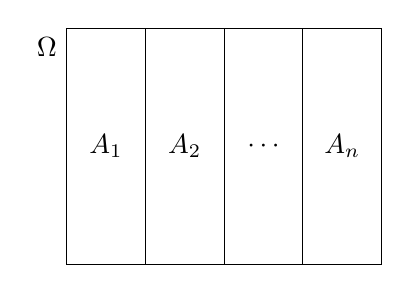
\begin{tikzpicture}
\draw (0,3) node[anchor=north east] {$\Omega$} rectangle (4,0);
\foreach \x in {1,2,3} {
	\draw (\x,0) -- (\x,3);
} 
\node at (0.5,1.5) {$A_1$};
\node at (1.5,1.5) {$A_2$};
\node at (2.5,1.5) {$\cdots$};
\node at (3.5,1.5) {$A_n$};
\end{tikzpicture}
\end{center}

Usually it's easy to get a partition of the sample space splitting a population according to some categorical variable,
like for example gender, blood type, etc.
\end{frame}


%---------------------------------------------------------------------slide----
\begin{frame}
\frametitle{Total probability theorem}
If we have a partition of a sample space, we can use it to calculate the probabilities of other events in the same
sample space.
\begin{theorem}[Total probability]
Given a partition $A_1,\ldots,A_n$ of a sample space $\Omega$, the probability of any other event $B$ of the same sample
space can be calculated with the formula
\[
P(B) = \sum_{i=1}^n P(A_i\cap B) = \sum_{i=1}^n P(A_i)P(B|A_i).
\]
\end{theorem}
\end{frame}


%---------------------------------------------------------------------slide----
\begin{frame}
\frametitle{Total probability theorem}
\framesubtitle{Proof}
The theorem proof is quite simple.
As $A_1,\ldots,A_n$ is a partition of $\Omega$, we have 
\[
B = B\cap \Omega = B\cap (A_1\cup \cdots \cup A_n) = (B\cap A_1)\cup \cdots \cup (B\cap A_n).
\]
And all the events of this union are mutually incompatible as $A_1,\ldots,A_n$ are, thus
\begin{align*}
P(B) &= P((B\cap A_1)\cup \cdots \cup (B\cap A_n)) = P(B\cap A_1)+\cdots + P(B\cap A_n) =\\
&= P(A_1)P(B|A_1)+\cdots + P(A_n)P(B|A_n) = \sum_{i=1}^n P(A_i)P(B|A_i).
\end{align*}

\begin{center}
\tikzsetnextfilename{probability/total_probability}
% Author: Alfredo Sánchez Alberca (asalber@ceu.es)

\begin{tikzpicture}
\def\ellipse {(2,1.5) ellipse (1.9cm and 1cm)};
\draw (0,3) node[anchor=north east] {$\Omega$} rectangle (4,0);
\foreach \x in {1,2,3} {
	\draw (\x,0) -- (\x,3);
};

\draw \ellipse;
\node at (2.5,2.2) {$B$};

\node at (0.5,0.2) {$A_1$};
\node at (1.5,0.2) {$A_2$};
\node at (2.5,0.2) {$\cdots$};
\node at (3.5,0.2) {$A_n$};


\pause
\begin{scope}
\clip (0,0) rectangle (1,3);
\draw[fill=color1!30] \ellipse;
\draw (1,0) -- (1,3);
\node[font=\scriptsize] at (0.6,1.5) {$A_1\cap B$}; 
\end{scope}
\pause
\begin{scope}
\clip (1,0) rectangle (2,3);
\draw[fill=color1!30] \ellipse;
\draw (1,0) -- (1,3);
\draw (2,0) -- (2,3);
\node[font=\scriptsize] at (1.5,1.5) {$A_2\cap B$}; 
\end{scope}
\pause
\begin{scope}
\clip (2,0) rectangle (3,3);
\draw[fill=color1!30] \ellipse;
\draw (2,0) -- (2,3);
\draw (3,0) -- (3,3);
\node at (2.5,2.2) {$B$};
\node[font=\scriptsize] at (2.5,1.5) {$\cdots$}; 
\end{scope}
\pause
\begin{scope}
\clip (3,0) rectangle (4,3);
\draw[fill=color1!30] \ellipse;
\draw (3,0) -- (3,3);
\node[font=\scriptsize] at (3.4,1.5) {$A_n\cap B$}; 
\end{scope}
\end{tikzpicture}
\end{center}
\end{frame}


%---------------------------------------------------------------------slide----
\begin{frame}
\frametitle{Total probability theorem}
\framesubtitle{Example of diagnosis}
A symptom $S$ can be caused by a disease $D$, but can also be present in persons without the disease.
In a population, the rate of people with the disease is $0.2$. 
We know also that $90\%$ of persons with the disease present the symptom, while only $40\%$ of persons without the
disease present it. 

\emph{What is the probability that a random person of the population presents the symptom?}

To answer the question we can apply the total probability theorem using the partition $\{A,\bar A\}$:
\[
P(S) = P(D)P(S|D)+P(\bar D)P(S/\bar D) = 0.2\cdot 0.9 + 0.8\cdot 0.4 = 0.5.
\]
That is, half of the population have the symptom. 

\begin{center}
\emph{Indeed, it is a weighted mean of probabilities!}
\end{center}
\end{frame}


%---------------------------------------------------------------------slide----
\begin{frame}
\frametitle{Total probability theorem}
\framesubtitle{Example of diagnosis with a tree diagram}
The answer to the previous question is even clearer with the tree diagram of the probabilistic space.

\begin{center}
\tikzsetnextfilename{probability/total_probability_space}
\resizebox{0.8\textwidth}{!}{% Author: Alfredo Sánchez Alberca (asalber@ceu.es)

\begin{tikzpicture}[
grow'=right,
% sloped,
level 1/.style ={level distance=2cm, sibling distance=1.6cm, parent anchor=east, child anchor=west},
level 2/.style ={level distance=2cm, sibling distance=0.8cm},
level 3/.style ={level distance=1.5cm, sibling distance=0.8cm, dashed},
level 4/.style ={level distance=3cm, sibling distance=0.8cm, dashed},
prob/.style={font=\footnotesize,above}
]


\node (root) {}
	child {node {$D$}
		child {node {$S$}
			child {node[color=color2]{$(D,S)$}
				child {node[color=color2]{$0.18$} edge from parent node[prob] {$0.2\cdot 0.9$}}
			}
			edge from parent node[prob] {$0.9$}
		}
		child {node {$\bar S$}
			child {node{$(D,\bar S)$}
				child {node{$0.02$} edge from parent node[prob] {$0.2\cdot 0.1$}}
			}
			edge from parent node[prob,below] {$0.1$}
		}
		edge from parent node[prob] {$0.2$}
	}
	child {node {$\bar D$}
		child {node {$S$}
			child {node[color=color2]{$(\bar D,S)$}
				child {node[color=color2]{$0.32$} edge from parent node[prob] {$0.8\cdot 0.4$}}
			}
			edge from parent node[prob] {$0.4$}
		}
		child {node {$\bar S$}
			child {node{$(\bar D,\bar S)$}
				child {node{$0.48$} edge from parent node[prob] {$0.8\cdot 0.6$}}
			}
			edge from parent node[prob,below] {$0.6$}
		}
		edge from parent node[prob,below] {$0.8$}
	};

\begin{scope}[every node/.style={text width=2cm, align=center, anchor=center, font=\bfseries,}]
\node[above= 0.5cm of root-1-1-1-1] (labels-level) {Probability};
\node[at =(labels-level-|root-1-1-1)] {$\Omega$};
\node[at =(labels-level-|root-1-1)] {Symptom};
\node[at =(labels-level-|root-1)] {Disease};
\end{scope}
\end{tikzpicture}
}
\end{center}

\begin{align*}
P(S) &= P(D,S) + P(\bar D,S) = P(D)P(S|D)+P(\bar D)P(S|\bar D)\\
& = 0.2\cdot 0.9+ 0.8\cdot 0.4 = 0.18 + 0.32 = 0.5.
\end{align*}
\end{frame}


\subsection{Bayes theorem}

%---------------------------------------------------------------------slide----
\begin{frame}
\frametitle{Bayes theorem}
A partition of a sample space $A_1,\cdots,A_n$ may also be interpreted as a set of feasible hypothesis to a fact
$B$.

In such cases may be helpful to calculate the posterior probability $P(A_i|B)$ of every hypothesis.

\begin{theorem}[Bayes]
Given a partition $A_1,\ldots,A_n$ of a sample space $\Omega$ and another event $B$ of the same sample space, the
conditional probability of every even $A_i$ $i=1,\ldots,n$ on $B$ can be calculated with the following formula
\[
P(A_i|B) = \frac{P(A_i\cap B)}{P(B)} = \frac{P(A_i)P(B|A_i)}{\sum_{i=1}^n P(A_i)P(B|A_i)}.
\]
\end{theorem}
\end{frame}


%---------------------------------------------------------------------slide----
\begin{frame}
\frametitle{Bayes theorem}
\framesubtitle{Example of diagnosis}
In the previous example, a more interesting question is about the diagnosis for a person with the symptom.  

In this case we can interpret $D$ and $\bar D$ as the two feasible hypothesis for the symptom $S$.
The prior probabilities for them are $P(D)=0.2$ and $P(D)=0.8$.
That means that if we don't have information about the symptom, the diagnosis would be that the person doesn't have the
disease.

However, if after examining the person we observe the symptom, that information changes the uncertainty about the
hypothesis, an we need calculate the posterior probabilities to diagnose, that is,
\[
P(D|S) \mbox{ y } P(\bar D|S)
\]
\end{frame}


%---------------------------------------------------------------------slide----
\begin{frame}
\frametitle{Teorema de Bayes theorem}
\framesubtitle{Example of diagnosis}
To calculate the posterior probabilities we can use the Bayes theorem.
\begin{align*}
P(D/S) &= \frac{P(D)P(S/D)}{P(D)P(S/D)+P(\bar D)P(S/\bar D)} = \frac{0.2\cdot 0.9}{0.2\cdot 0.9 + 0.8\cdot 0.4} = \frac{0.18}{0.5}=0.36,\\
P(\bar D/S) &= \frac{P(\bar D)P(S/\bar D)}{P(D)P(S/D)+P(\bar D)P(S/\bar D)} = \frac{0.8\cdot 0.4}{0.2\cdot 0.9 + 0.8\cdot 0.4} = \frac{0.32}{0.5}=0.64.
\end{align*}

As we can see the probability of having the disease has increased. 
Nevertheless, the probability of not having the disease is still greater than the probability of having it, and for that
reason, the diagnosis is not having the disease. 

In this case it is said the the symptom $S$ is \emph{not decisive} in order to diagnose the disease.
\end{frame}

% \subsection{Tests diagnósticos}
% 
% %---------------------------------------------------------------------slide----
% \begin{frame}
% \frametitle{Tests diagnósticos}
% En epidemiología es común el uso de tests para diagnosticar enfermedades.
% 
% Generalmente estos tests no son totalmente fiables, sino que hay cierta probabilidad de acierto o fallo en el diagnóstico, que suele
% representarse en la siguiente tabla:
% \begin{center}
% \begin{tabular}{|m{3cm}<{\centering}|m{3.5cm}<{\centering}|m{3.5cm}<{\centering}|}
% \cline{2-3}
% \multicolumn{1}{c|}{} & Presencia de la\newline enfermedad ($E$) & Ausencia de la\newline enfermedad ($\overline E$)\\ \hline
% Test positivo\newline ($+$) & \textcolor{green}{Diagnóstico acertado\newline  $P(+/E)$}\qquad
% \highlight{Sensibilidad}& \textcolor{red}{Diagnóstico erróneo\newline $P(+/\overline E)$}\\ \hline Test negativo\newline ($-$) &
% \textcolor{red}{Diagnóstico erróneo\newline $P(-/E)$} & \textcolor{green}{Diagnóstico acertado\newline $P(-/\overline
% E)$}\qquad \highlight{Especificidad}\\ \hline
% \end{tabular}
% \end{center}
% 
% \note{
% En epidemiología es común el uso de tests para diagnosticar enfermedades.
% 
% Generalmente estos tests no son totalmente fiables, sino que hay cierta probabilidad de acierto o fallo en el diagnóstico, que suele
% representarse en la siguiente tabla:
% \begin{center}
% \begin{tabular}{|m{3cm}<{\centering}|m{3.5cm}<{\centering}|m{3.5cm}<{\centering}|}
% \cline{2-3}
% \multicolumn{1}{c|}{} & Presencia de la\newline enfermedad ($E$) & Ausencia de la\newline enfermedad ($\overline E$)\\ \hline
% Test positivo\newline ($+$) & \textcolor{green}{Diagnóstico acertado\newline  $P(+/E)$}\newline\highlight{Sensibilidad}& \textcolor{red}{\noindent Diagnóstico erróneo\newline $P(+/\overline E)$}\\ \hline
% Test negativo\newline ($-$) & \textcolor{red}{Diagnóstico erróneo\newline $P(-/E)$} & \textcolor{green}{Diagnóstico acertado\newline $P(-/\overline E)$}\newline\highlight{Especificidad}\\ \hline
% \end{tabular}
% \end{center}
% }
% \end{frame}
% 
% 
% 
% %---------------------------------------------------------------------slide----
% \begin{frame}
% \frametitle{Tests diagnósticos}
% La valided de una prueba diagnóstica depende de estas dos probabilidades:
% \begin{description}
% \item[\textbf{Sensibilidad}] Es el porcentaje de positivos entre las personas enfermas: $P(+/E)$.
% \item[\textbf{Especificidad}] Es el porcentaje de negativos entre las personas sanas: $P(-/\bar E)$.
% \end{description}
% 
% Pero lo realmente interesante de un un test diagnóstico es su capacidad predictiva para diagnosticar, lo cual se mide mediante las
% siguientes probabilidades a posteriori:
% \begin{description}
% \item[\textbf{Valor predictivo positivo}] Es el porcentaje de enfermos entre los positivos: $P(E/+)$.
% \item[\textbf{Valor predictivo negativo}] Es el porcentaje de sanos entre los negativos: $P(\bar E/-)$.
% \end{description}
% 
% Sin embargo, estos últmos valores dependen del porcentaje de enfermos en la población $P(E)$, lo que se conoce como, \highlight{\textbf{tasa
% o prevalencia}} de la enfermedad.
% 
% \note{
% La valided de una prueba diagnóstica depende de estas dos probabilidades:
% \begin{description}
% \item[Sensibilidad] Es el porcentaje de positivos entre las personas enfermas: $P(+/E)$.
% \item[Especificidad] Es el porcentaje de negativos entre las personas sanas: $P(-/\bar E)$.
% \end{description}
% 
% Pero lo realmente interesante de un un test diagnóstico es su capacidad predictiva para diagnosticar, lo cual se mide mediante las
% siguientes probabilidades a posteriori:
% \begin{description}
% \item[Valor predictivo positivo] Es el porcentaje de enfermos entre los positivos: $P(E/+)$.
% \item[Valor predictivo negativo] Es el porcentaje de sanos entre los negativos: $P(\bar E/-)$.
% \end{description}
% 
% Sin embargo, estos últimos valores dependen del porcentaje de enfermos en la población $P(E)$, lo que se conoce como,
% \highlight{\textbf{tasa o prevalencia}} de la enfermedad.
% }
% \end{frame}
% 
% 
% % ---------------------------------------------------------------------slide----
% \begin{frame}
% \frametitle{Tests diagnósticos}
% \frametitle{Ejemplo}
% Un test para diagnosticar la gripe tiene una sensibilidad del $95\%$ y una especificidad del $90\%$. Según esto, las probabilidades de
% acierto y fallo del test son:
% \begin{center}
% \begin{tabular}{|c|c|c|}
% \cline{2-3}
% \multicolumn{1}{c|}{} & Gripe & No gripe\\ \hline
% Test $+$ & \textcolor{green}{$0.95$} & \textcolor{red}{$0.10$}\\ \hline
% Test $-$ & \textcolor{red}{$0.05$} & \textcolor{green}{$0.90$}\\ \hline
% \end{tabular}
% \end{center}
% 
% Si la prevalencia de la gripe en la población es del $10\%$ y al aplicar el test a un individuo da positivo, \emph{¿cuál es la probabilidad
% de que tenga gripe?}
% 
% Aplicando el teorema de Bayes, se tiene que el valor predictivo positivo del test vale
% \begin{align*}
% P(\mbox{Gripe}/+) &= \frac{P(\mbox{Gripe})P(+/\mbox{Gripe})}{P(\mbox{Gripe})P(+/\mbox{Gripe})+P(\overline{\mbox{Gripe}})P(+/\overline{\mbox{Gripe}})} =\\
% &= \frac{0.1\cdot 0.95}{0.1\cdot 0.95+0.9\cdot 0.1} = 0.5135.
% \end{align*}
% Aunque con esta probabilidad se diagnosticaría la enfermedad en caso de que el test diese positivo, se trata de un valor predictivo positivo
% muy bajo. 
% 
% \note{
% Veamos un ejemplo. 
% 
% Un test para diagnosticar la gripe tiene una sensibilidad del $95\%$ y una especificidad del $90\%$. Según esto, las probabilidades de
% acierto y fallo del test son:
% \begin{center}
% \begin{tabular}{|c|c|c|}
% \cline{2-3}
% \multicolumn{1}{c|}{} & Gripe & No gripe\\ \hline
% Test $+$ & \textcolor{green}{$0.95$} & \textcolor{red}{$0.10$}\\ \hline
% Test $-$ & \textcolor{red}{$0.05$} & \textcolor{green}{$0.90$}\\ \hline
% \end{tabular}
% \end{center}
% 
% Si la prevalencia de la gripe en la población es del $10\%$ y al aplicar el test a un individuo da positivo, \emph{¿cuál es la probabilidad
% de que tenga gripe?}
% 
% Aplicando el teorema de Bayes, se tiene
% \begin{align*}
% P(\mbox{Gripe}/+) &= \frac{P(\mbox{Gripe})P(+/\mbox{Gripe})}{P(\mbox{Gripe})P(+/\mbox{Gripe})+P(\overline{\mbox{Gripe}})P(+/\overline{\mbox{Gripe}})} =\\
% &= \frac{0.1\cdot 0.95}{0.1\cdot 0.95+0.9\cdot 0.1} = 0.51.
% \end{align*}
% 
% La probabilidad de no tener la gripe sería $1-0.51=0.49$ ya que es el suceso contrario de tener la gripe, y como la probabilidad de tener la
% gripe es mayor que la de no tenerla, se diagnosticaría que tiene gripe. Sin embargo, el valor predictivo positivo de este test es muy bajo y
% nos equivoaríamos en el 49\% de los diagnósticos de enfermedad.
% }
% \end{frame}
% 
% 
% % ---------------------------------------------------------------------slide----
% \begin{frame}
% \frametitle{Tests diagnósticos}
% \frametitle{Ejemplo}
% \begin{center}
% \begin{tabular}{|c|c|c|}
% \cline{2-3}
% \multicolumn{1}{c|}{} & Gripe & No gripe\\ \hline
% Test $+$ & \textcolor{green}{$0.95$} & \textcolor{red}{$0.10$}\\ \hline
% Test $-$ & \textcolor{red}{$0.05$} & \textcolor{green}{$0.90$}\\ \hline
% \end{tabular}
% \end{center}
% 
% Y si el test da negativo, \emph{¿cuál es la probabilidad de que no tenga gripe?}
% 
% De nuevo, aplicando el teorema de Bayes, se tiene que el valor predictivo negativo del test vale
% \begin{align*}
% P(\overline{\mbox{Gripe}}/-) &=
% \frac{P(\overline{\mbox{Gripe}})P(-/\overline{\mbox{Gripe}})}{P(\mbox{Gripe})P(-/\mbox{Gripe})+P(\overline{\mbox{Gripe}})P(-/\overline{\mbox{Gripe}})}
% =\\ &= \frac{0.9\cdot 0.9}{0.1\cdot 0.05+0.9\cdot 0.9} = 0.9939.
% \end{align*}
% De manera que el valor predictivo negativo de este test es mucho más alto que el valor predictivo positivo.
% 
% \note{
% Y si el test da negativo, \emph{¿cuál es la probabilidad de que no tenga gripe?}
% 
% De nuevo, aplicando el teorema de Bayes, se tiene que el valor predictivo negativo del test vale
% \begin{align*}
% P(\overline{\mbox{Gripe}}/-) &=
% \frac{P(\overline{\mbox{Gripe}})P(-/\overline{\mbox{Gripe}})}{P(\mbox{Gripe})P(-/\mbox{Gripe})+P(\overline{\mbox{Gripe}})P(-/\overline{\mbox{Gripe}})}
% =\\ &= \frac{0.9\cdot 0.9}{0.1\cdot 0.05+0.9\cdot 0.9} = 0.9939.
% \end{align*}
% De manera que el valor predictivo negativo de este test es mucho más alto que el valor predictivo positivo, y por tanto este test es mucho
% más útil para descartar la enfermedad que para detectarla. 
% }
% \end{frame}


